\chapter{Predchádzajúce riešenia}\label{chap:previous_solutions}

Existuje mnoho prác, ktoré sa zaoberajú sledovaním ruky v obraze. Je veľké množstvo metód, ktoré sa používajú v závislosti na vstupných dátach a dostupných hardvérových prostriedkoch. Väčšina prác uvažuje obraz, na ktorom je ruka ako prvý a najväčší objekt. Postupom času sa výskum rozšíril na vytvorenie systému, ktorý je schopný detegovať pozície niekoľkých rúk na obraze. Veľký pokrok priniesli aj do tejto oblasti konvolučné neurónové siete. % a metóda hlbokého učenia.
Vďaka nim je možné presnejšie určovať pozíciu jednej a viacerých rúk. Ďalším pokrokom bolo rozlišovanie medzi prstami, teda je možné presne párovať kĺb ruky na súradnice v obraze.

V tejto kapitole popíšeme tri práce, ktoré pristupujú k určovaniu pozície ruky rôznymi spôsobmi. Výber týchto prác je vhodný aj preto, že používajú vstupné dáta, ktoré sú v podobnej forme ako dáta z kamery použitej v našej práci. Systémy navrhnuté v týchto troch riešeniach by bolo možné použiť ako učenie robota s ľudským učiteľom, čo prispieva k vyhodnoteniu najlepšieho prístupu a porovnanie pre riešenie v tejto oblasti. Taktiež tieto práce poskytujú implementované riešenia a bolo možné zreprodukovať ich dosiahnuté výsledky.

\section{Sledovanie ruky z RGB-D dát bez CNN}\label{chpt:depthBase}
Sledovanie a určovanie polohy ruky na RGB-D dátach je možné aj bez použitia konvolučných neurónových sietí. Stan Melax a kol. \cite{DBLP:journals/corr/MelaxKO17} použili vo svojej práci hĺbkové dáta, na ktoré mapovali syntetickú ruku. Použitím správneho predspracovania dát dosiahli úspešné odhadovanie polohy ruky. 

Sledovací algoritmu je možné používať v reálnom čase. Sleduje plne definovaný 3D model ruky. Systém využíva predošlú pozíciu ruky, ktorú na ďalšom snímku videa upraví. Syntetický model ruky je definovaný ako konvexné pevné teleso, čo umožňuje priblížiť sa k zachytenej ruke na obraze.

Mračná bodov získané z hĺbkového senzora kamery obsahujú tisícky bodov.Väčšinou sú tieto body namerané správne, ale senzor niekedy zaznamená nesprávnu informáciu. Pri rýchlych pohyboch však nie je možné a ani potrebné, aby bola pozícia modelu upravená podľa každého nameraného bodu. Preto zredukovali tieto dáta na minimálny počet, ktorý jednoznačne definuje pozíciu ruky v obraze. Pre niektoré pixely však vypočíta a vráti nesprávnu vzdialenosť od kamery, čo spôsobuje uloženie ruky v neprirodzených polohách. Odstránením šumu a týchto nesprávnych bodov boli získané lepšie výsledky a sledovací algoritmus bol rýchlejší. Toto zlepšenie bolo dosiahnuté implementáciou pod-vzorkovania voxelov do mriežky. Pre každý voxel bolo vypočítané ťažisko, ktoré reprezentuje skupinu hĺbkových dát.

Model ruky má na začiatku prednastavenú prirodzenú polohu. Využíva vlastnosti pevných telies pri zmene polohy kľúčových bodov na ruke, vďaka čomu sa udrží v prirodzenej póze. Hĺbkové dáta z kamery vplývajú na model tak, že poloha modelu je upravená podľa ľudskej ruky pred kamerou. Pozícia vyššie spomínaného ťažiska voxelu je použitá ako kľúčový bod ovplyvňujúci jednotlivé časti modelu ruky. Úprava syntetickej ruky má magnetické správanie, teda najbližší kľúčový bod syntetickej ruky je posunutý k najbližšiemu ťažisku.

So senzoru sú získavané aj informácie o miestach, kde sa objekt nenachádza. Tieto oblasti označili ako priestor kolíznych hraníc 3D modelu ruky a zabránili posunu model do týchto oblastí. Pretože malé objekty ako prsty sa môžu pohybovať relatívne rýchlo k ich veľkosti, nepridávali im blokovací kolízny priestor, keďže požiadavkou bol voľný pohyb k dosiahnutiu čo najvyššej presnosti.

Pri tomto systéme občas dochádza k nesprávnej identifikácii prstov. Používateľ môže napríklad ukazovať iba jedným prstom (ukazovákom), ale systém namapuje na hĺbkové dáta iný prst, napr. prostredník alebo palec. Môže nastať aj prípad, že z mračna bodov je potenciál na viac zdvihnutých prstov ale lokálna príťažlivosť modelu na tieto body zabraňuje zdvihnúť alebo schovať nadbytočný prst. Na vyriešenie tohoto problému Stan Meax a kol. \cite{DBLP:journals/corr/MelaxKO17} vychádzali z predošlého najlepšie priradeného modelu. Pretože najlepšie mapovanie modelu na hĺbkové dáta môže trvať niekoľko snímkov, výber prstov pri taktomto rozhodovaní sa vykoná každú pol sekundu.

\subsection{Syntetický model ruky}
Model ruky vymodelovali z 3 častí pre každý prst a jednej časti dlane. Model je zobrazený na obr. \ref{img:41handModel}. Každá časť bola definovaná ako pevné teleso a teda zachováva aj vlastnosti a výpočet kolízií pevných telies. Taktiež majú pevné telesá pridelené kosti, ktoré im upravujú pohyb. Model je reprezentovaný súborom exportovaným z programu 3DS Max. Dôležitá je veľkosť modelu, ktorá bola zvolená na takú, aby systém fungoval s väčšinou bežných dospelých ľudských rúk teda na dĺžku 20cm. Existujú techniky, ktoré automaticky preškálujú model podľa potreby, čo ale nie je cieľom tejto práce a prednastavená jedna veľkosť modelu je dostačujúca pre tento výskum.

\begin{figure}[H]
	\begin{center}
		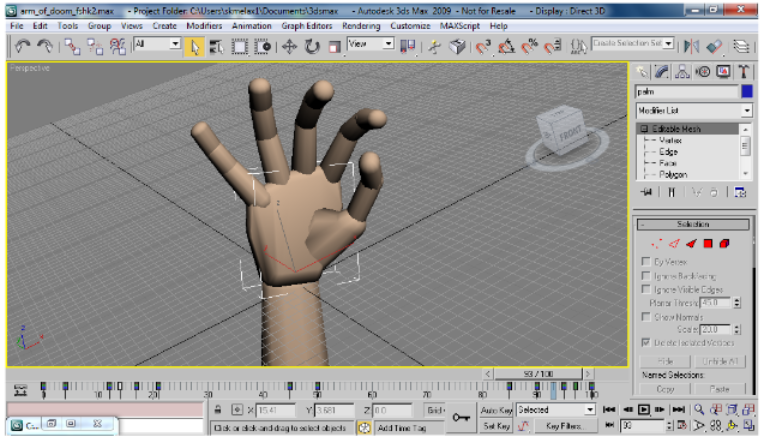
\includegraphics[height=\imageHeight]{images/41handModel.png}
		\caption{Model ruky v 3DS Max}
		\label{img:41handModel}
	\end{center}
\end{figure}

\subsection{Výpočet chyby}
Stan Meax a kol. \cite{DBLP:journals/corr/MelaxKO17} použili meranie vzdialenosti medzi množinou bodov na modeli ruky a príslušnému bodu na používateľovej ruke. Nakoľko hĺbkové dáta znázorňujúce používateľovu ruku nie sú jednoznačné, nedá sa určiť, ktoré prislúchajú ktorým bodom syntetickej ruky. Známe je, že ak existuje bod v hĺbkových dátach $P$ a je daná vzdialenosť od povrchu sledovaného modelu $B$, potom model musí byť posunutý aspoň o vzdialenosť, ktorá súhlasí s aktuálnym stavom používateľovej ruky. Vzdialenosť chyby je zobrazená červenými úsečkami na obr. \ref{img:42erroMesurement}. Definovanie chyby vychádza z tohoto predpokladu. Teda pre každé pevné teleso $B_i$ v modeli $B$ je nájdená minimálna vzdialenosť o ktorú musí byť posunutý model pre najlepšiu zhodnú pozíciu s hĺbkovými dátami. V hĺbkových dátach je vybrané mračno bodov $P_i$, ktoré sú najbližšie k povrchu pevného telesa $B_i$. Priebeh výpočtu je nasledovný:

\begin{equation}\label{eqn:distance}
    P_i=\{p:p\in P, min\{|p-b_i|:b_i\in B_i\} = min\{|p-b|:b\in B\}\}
\end{equation}

Následne sa z tejto množiny vyberie najvzdialenejší bod $p$. Vzdialenosť je potom vypočítaná medzi bodom $p$ a k nem najbližšiemu bodu $b$ z pevného telesa $B_i$, ku ktorému bolo vybrané príslušné mračno bodov $P_i$. Celý výpočet tejto chyby môžeme zapísať takto:
%Definovali to ako vzdialenosť od najvzdialenejšieho bodu $p$ v množine mračnových bodov $P_i$, ktoré sú najbližšie k povrchu pevného telesa $B_i$ ako je znázornené na (\ref{eqn:errFitt})

\begin{equation}\label{eqn:errFitt}
    errFitt_i = max\{min\{|p-b_i|:b_i\in B\}:p\in P_i\}
\end{equation}

\begin{figure}[H]
	\begin{center}
		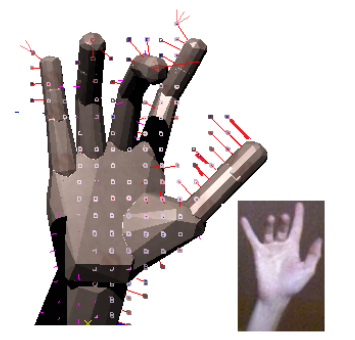
\includegraphics[height=\imageHeight]{images/42erroMesurement.png}
		\caption{Ovplyvnenie 3D modelu ruky hĺbkovými dátami. Vybrané body $p$ z mračna bodov sú znázornené tmavými bodkami, z ktorých vychádzajú červené úsečky.Tie vyjadrujú vzdialenosť medzi bodom $p$ a najbližším bodom modelu ruky $b$. Túto vzdialenosť vypočítame ako na (\ref{eqn:errFitt})}.
		\label{img:42erroMesurement}
	\end{center}
\end{figure}

K chybe podľa (\ref{eqn:errFitt}) sa pričíta ešte chyba za nesprávne zvolenú pozíciu pevného telesa (\ref{eqn:penalty}). Miesta pre penalizáciu sú tie, kde hĺbkové dáta nezachytili žiaden objekt, teda sa tam v skutočnosti nič nemôže nachádzať. Vzali centroid každej kosti, ktorý sa neprekrýva s pixelmi hĺbkových dát. Chyba je aspoň taká veľká ako polomer najväčšej vpísanej gule.

\begin{equation}\label{eqn:penalty}
    errOcc_i = 
    \begin{cases}
        r, & \text{ak sa centroid ($B_i$) prekrýva s pozadím}\\
        0, & \text{inak}
    \end{cases}
\end{equation}

Celková chyba je potom vypočítaná ako súčet chyby a penalizácie každého pevného telesa (\ref{eqn:errTotal}). Kde $errFit$ je množina chýb a $errOcc$ je množina penalizácií, kde každá chyba alebo penalizácia prislúcha práve jednému pevnému telesu $B_i$ z celého modelu ruky $B$.

\begin{equation}\label{eqn:errTotal}
    errTotal=\sum{err_i \in errFit} + \sum{err_i \in errOcc}
\end{equation}

\subsection{Vyhodnotenie}
Tento systém je schopný sledovať ruku na základe hĺbkových dát a každému kĺbu prideliť pozíciu v 3D priestore. Keďže hĺbkové dáta najbližšie ku kamere sú predpokladom na určenie pozície ruky, tak musí byť prvým objektom pred kamerou ruka aby systém fungoval, čo prináša isté obmedzenia.

Na jeho používanie a sledovanie ruky v reálnom čase stačí jeden procesor pre jednoduchšie pózy. So zvyšujúcim výkonom hardvéru je možné plynule sledovať zložitejšie polohy. Aby bolo možné sledovať viac rúk, systému by stačilo pridať rozdelenie hĺbkových dát do skupín napr. algoritmom `k-means clustering", čím by sa odlišovalo medzi rukami.

\section{Sledovanie ruky z RGB dát s CNN}\label{chpt:GANerated}
Najbežnejšie rozšírenými vstupnými dátami sú RGB obrázky. Vytvorenie takýchto snímkov je dnes jednoduché a dostupné takmer každému. Problémom je však určiť pozíciu konkrétnych bodov v 3D priestore, pretože nemáme informáciu o vzdialenosti k danému bodu. Navyše nie je možné túto vzdialenosť vypočítať z jedného obrázku. Myšlienkou ako vyriešiť tento problém a získať informáciu o vzdialenosti od kamery je pridanie syntetického modelu sledovaného objektu, ktorý je vložený do obrázka na základe bodov definovaných v dvoch dimenziách. Nájdením pozície ruky v 3D priestore z jedného RGB obrázka sa zaoberala Franziska Mueller a kol. \cite{GANeratedHands_CVPR2018}

Vytvorili systém, ktorý v reálnom čase sleduje polohu ruky z RGB obrázku. Tok videa je posielaný do CNN, ktorá funguje na princípe regresie kĺbov ruky. Táto sieť {\it RegNet} predikuje 2D a 3D pozíciu 21 kĺbov. 2D pozícia je reprezentovaná tepelnými mapami a 3D pozície sú reprezentované relatívnymi 3D súradnicami voči zápästiu.

{\it RegNet} zobrazená na obr. \ref{img:43GANerated} využíva reziduálnu sieť, ktorá pozostáva z 10 reziduálnych blokov odvodených z architektúry {\it ResNet50} \cite{DBLP:journals/corr/HeZRS15}. Pre zlepšenie prepojenia 2D a 3D predikcie pridali projekčnú vrstvu {\it ProjLayer}. Myšlienka za touto vrstvou je vytvoriť tzv. ortografickú projekciu 3D predikcie, z ktorej je vytvorená 2D Gausovská tepelná mapa. Tieto mapy vplývajú na zvyšnú časť siete pre dosiahnutie finálnej 2D a 3D predikcie. V práci ukázali, že táto vrstva prispela ku zlepšeniu výsledkov.

\begin{figure}[H]
	\begin{center}
		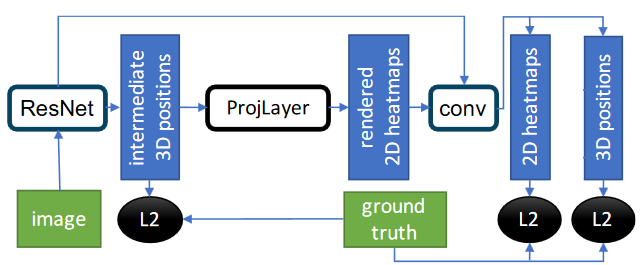
\includegraphics[height=\imageHeight]{images/43GANerated.png}
		\caption{Architektúra {\it RegNet}\cite{GANeratedHands_CVPR2018}. ResNet a conv sú trénovateľné, chyba sa spätne šíri cez ProjLayer. Vstupné dáta sú označené zelenou a generované dáta sieťou sú označené modrou farbou. Časti cenovej funkcie sú zobrazené v čiernych ováloch.}
		\label{img:43GANerated}
	\end{center}
\end{figure}

\subsection{Dataset}
Anotovanie rúk v 3D priestore pre skutočné fotografie je veľmi náročné, preto použili vygenerované obrázky rôznych polôh počítačom vytvorenej syntetickej ruky. Výhodou takých obrázkov je známa pozícia kĺbov. Rozdiely medzi skutočnou a syntetickou rukou však limitujú generalizačnú schopnosť CNN. Aby sieť vedela predikovať aj snímky so skutočného sveta, tak sú potrebné trénovacie obrázky aj z reálneho sveta. Dôležité je, aby syntetické a reálne obrázky navzájom nezobrazovali rovnaký snímok.

Aby použili reálne vyzerajúce obrázky a mali aj 3D pozíciu každého kĺbu, vytvorili generátor obrázkov na základe teórie podľa Goodfellow a kol. \cite{Goodfellow-et-al-2016}. Využíva myšlienku teórie hry, v ktorej musí generátor súťažiť voči diskriminačnej sieti. Generovaný je priamo vzorový obrázok a diskriminačná sieť určí pravdepodobnosť, že tento obrázok je skôr skutočným trénovacím vstupom než vygenerovaným obrázkom. Cieľom je maximalizovať pravdepodobnosť, že generovaný obrázok je skutočným vstupom.

Sieť na generovanie obrázkov, ktorej teoretický základ je popísaný vyššie, navrhli \cite{GANeratedHands_CVPR2018} tak, aby zo syntetického obrázka vytvorila reálny a opačne. Vstupom do siete sú dvojice syntetickej a reálnej ruky na bielom pozadí. Pre každý obrázok je aplikovaná funkcia na vytvorenie syntetického alebo reálneho páru pre vstup. Kontrolovanie konzistencie prebieha spätným vytvorením pôvodného obrázka a porovnaním L1 normou. Upravený obrázok je vstupom do binárneho klasifikátora, ktorý určuje pre každý pixel, či patrí pozadiu alebo ruke. Takto vytvorená silueta je porovnaná so siluetou pôvodného obrázka krížovou entrópiou. Táto sieť je trénovaná na SynthHand \cite{DBLP:journals/corr/MuellerMS0CT17} datasete a vlastnom datasete rúk, ktoré sú zachytené na zelenom pozadí. Architektúra je ilustrovaná na obr. \ref{img:generateHands}.

\begin{figure}[H]
	\begin{center}
		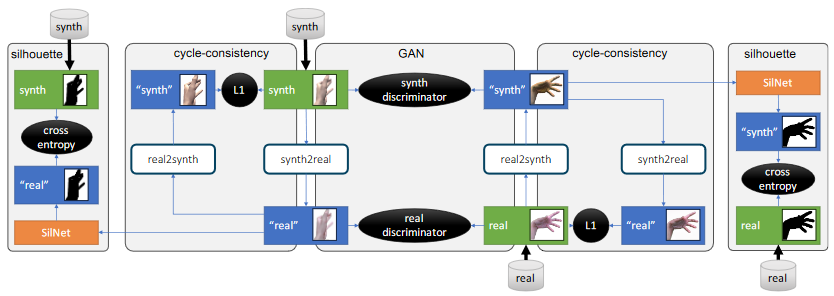
\includegraphics[width=\textwidth]{images/GenerateHands.png}
		\caption{Architektúra siete na generovanie obrázkov \cite{GANeratedHands_CVPR2018}. V bielych obdĺžnikoch sú trénovateľné časti, čiernou sú označené stratové funkcie, zelenou sú obrázky z datasetu, modrou sú označené vygenerované obrázky a oranžovou binárny klasifikátor.}
		\label{img:generateHands}
	\end{center}
\end{figure}

Natrénovaná sieť je potom použitá na vytvorenie reálne vyzerajúcich obrázkov z rôznych póz vymodelovanej ruky so známimi 3D súradnicami. Syntetickým obrázkom menili pozadie náhodnými textúrami a aj úplne náhodnými farbami. Výstupom zo siete je RGB obrázok s 3D pozíciami kĺbov reálnej ruky.

\subsection{Model ruky a jeho umiestnenie v obrázku}
Získaním predikcie 2D tepelných máp a 3D súradníc z CNN boli schopní \cite{GANeratedHands_CVPR2018} umiestniť kinematickú kostru pre tieto dáta. Predikované pozície sú také, že umiestnenie kostry podľa nich zobrazuje polohu, ktorú človek dokáže napodobniť.

Syntetický model ruky je zložený zo zápästia reprezentovaného základným kĺbom (ostatné kĺby majú relatívnu polohu k tomuto kĺbu v 3D súradniciach) a 20 kĺbmi prstov, vrátane končekov prstov, ktoré majú nulový stupeň voľnosti. Ostatných 15 kĺbov prstov má stupeň voľnosti jeden alebo dva. Absolútna poloha kĺbu je určená ako $\Theta = (t, {\bf R}, \theta)$, kde $t \in \mathbb{R}^3$, a ${\bf R} \in SO(3)$ je globálna pozícia a rotácia zápästného kĺbu, a $\theta \in \mathbb{R}^{20}$ je vektor uhlov desiatich kĺbov so stupňom voľnosti jedna a piatich kĺbov so stupňom voľnosti dva. Ako globálny súradnicový systém brali do úvahy súradný systém kamery.

Pre správne umiestnenie kostry je úlohou minimalizovať chybu definovanú ako $E(\Theta) = E_{2D}(\Theta) + E_{3D}(\Theta) + E_{limit}(\Theta) + E_{temp}(\Theta) $. Trénovaním 2D tepelnej mapy je účelom minimalizovať vzdialenosť medzi pozíciou kĺbu projektovanú v obraze a maximálnou hodnotou v prislúchajúcej tepelnej mape. Matematicky zapísané na rovnici (\ref{eqn:E2D}).
\begin{equation}\label{eqn:E2D}
    E_{2D}(\Theta) = \sum_j \omega_j ||\Pi(\mathcal{M}_j(\Theta)) - u_j||_2^2
\end{equation}
Kde $u_j \in \mathbb{R}^2$ označuje maximálnu hodnotu v tepelnej mape pre j-ty kĺb, $\omega_j > 0$ je skalár označujúci váhu odvodenú z tepelnej mapy a $\Pi:\mathbb{R}^3 \mapsto \mathbb{R}^2$ je projekcia z 3D priestoru na 2D obrázkovú plochu. Túto projekciu ovplyvňuje nastavenie kamery. Výstup z 3D regresie je relatívnou polohou k zápästiu.

\subsection{Vyhodnotenie}

Na vyhodnocovanie presnosti predikcie a porovnanie z inými prístupmi k predikcii ruky v obraze sa počítali percentá správne určených kĺbov. Správne určenie kĺbu je vtedy, ak jeho predikovaná pozícia leží v kružnici pre 2D a v guli pre 3D prípad so stredom v súradniciach očakávanej pozície kĺbu a priemerom 50 mm. Vyhodnocovaním týmto spôsobom na čisto syntetických dátach dosiahli presnosť 55\%. Pridaním reálne vyzerajúcich obrázkov a rozdelením trénovacej a testovacej množiny dosiahol presnosť 96.5\% na Stereo datasete \cite{DBLP:journals/corr/ZhangJCQXY16}.

\section{Detekcia 3D polohy ruky s použitím architektúry Hourglass}\label{chpt:hourglass}

Ďalšou možnosťou ako pristupovať k problému hľadania polohy ruky v obraze je vytvoriť vhodnú architektúru neurónovej siete tak, aby na vstupe mala jeden hĺbkový obrázok, pre ktorý určí pozície kĺbov ruky v 3D priestore. Tento spôsob využil Fuyang a kol. \cite{DBLP:journals/corr/hourglass}, ktorých návrh a implementáciu popisuje táto podkapitola, pričom architektúru siete vytvorili podľa siete Hourglass na základe výsledkov riešenia podobného problému určovania polohy človeka, ktorým sa zaoberal Newell a kol. \cite{DBLP:journals/corr/NewellYD16}.

\subsection{Návrh metódy}
Navrhli systém založený na regresnom prístupe (podsekcia \ref{subchapt:regression_approach}), ktorý pracuje s hĺbkovým obrázkom. Vstupom do systému je normalizovaný binárny voxel a na výstupe je 3D tepelná mapa kĺbov v pirestore voxelov. Vstupný obrázok je najprv premietnutý do súradnicového priestoru kamery ako mračno bodov. Následne je toto mračno prevedené na diskrétne binárne voxely normalizované podľa veľkosti mračna bodov. Trénovacím výstupom je 3D Gaussovo rozdelenie pravdepodobností výskytu kĺbov ako tepelná mapa pre každý kĺb. Súčasne je trénovaná sieť na vytváranie tepelnej mapy 3D kostí. Vďaka nej je možné zahrnúť závislosť medi kĺbmi na ruke a kosťami, ktoré tieto kĺby prepájajú. Tento návrh je zobrazený na Obr. \ref{img:FuyangFramework} \cite{DBLP:journals/corr/hourglass}.

\begin{figure}[H]
	\begin{center}
		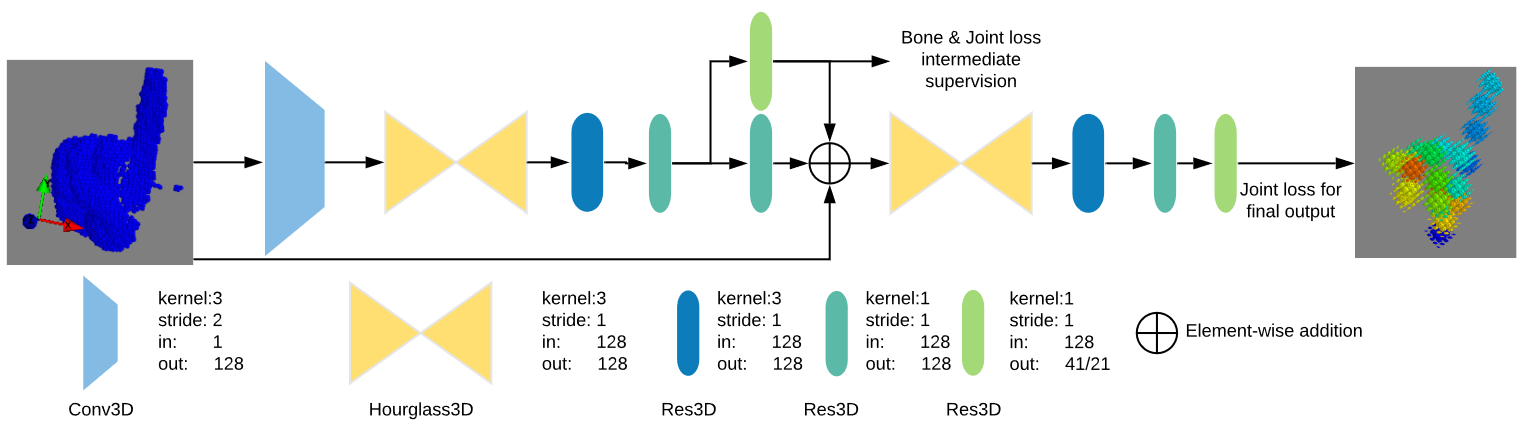
\includegraphics[width=\textwidth]{images/231hourglass.png}
		\caption{Návrh systému s použitím 2 modulov architektúry siete Hourglass}
		%. Zobrazuje tieto dva za sebou zapojené moduly znázornené dvoma žltými trojuholníkmi. Na vstupe sú diskrétne objemové dáta zobrazené modrým kvádrom. Tie sú podvzorkované jadrom 3x3 a krokom 2. Medzi modulmi Hourglass je Res3D modul s jadrom 3x3 a Res3D s jadrom 1x1, z ktorých sú generované tepelné mapy kostí a kĺbov.}
		\label{img:FuyangFramework}
	\end{center}
\end{figure}

\subsection{Predspracovanie dát}\label{hourglass:preprocessing}
Vstupné dáta do modulu Hourglass sú upravené do objemovej reprezentácie a sú premietnuté do priestoru kamery podľa vnútorných parametrov kamery. Vytvárajú mračno bodov, ktoré je zjednodušené na mračno bodov ohraničené kvádrom. Na vytvorenie takého ohraničenia sa v tejto metóde používa geometrický stred bodov mračna a rozmery ako najvzdialenejšie body v osiach x, y, z. Potom je mračno bodov prevedené do diskrétneho priestoru binárnej mriežky voxelov. Ak je voxel označený jednotkou, obsahuje hĺbkové dáta inak je označený nulou.
Očakávané súradnice pre kĺby vyjadrujú iba jeden bod v priestore. Teda je distribúcia týchto bodov veľmi riedka pre tréning. Zväčšenie množstva týchto bodov je dosiahnuté 3D Gaussovou distribúciou v okolí súradníc kĺbu so stredom v jeho súradniciach a smerodajnou odchýlkou dĺžky mriežky. Táto distribúcia vyjadruje tepelnú mapu očakávaných súradníc. Príklad takejto mapy je znázornený na obr. \ref{img:FuyangFramework}.

\subsection{Štruktúra siete}
Základným modulom je Hourglass sieť, ktorej architúru sme popísali v \ref{architecture_hourglass}. Podľa návrhu má táto sieť pracovať s 3D dátami, a preto vrstvy v tomto module sú upravené tak, aby používali 3D konvolučné vrstvy. Výpočty týchto vrstiev je náročnejšie vykonať a viac údajov sa musí uložiť do pamäte. Preto je znížené rozlíšenie vstupných voxelov na 64x64x64 a výstupne rozlíšenie z modulu hourglass na 32x32x32. Na vybudovanie siete boli použité dva takéto moduly, kde výstup z prvého modulu je použitý aj na vygenerovanie tepelnej mapy kostí a kĺbov. Táto časť je tvorená z tzv. Res3D modulu s jadrom 3x3 a dvoma Res3D modulmi s jadrom 1x1. Vstupom do druhého hourglass modulu je súčet pôvodného vstupu, výstupu z prvého hourglass modulu a z tepelnej mapy kostí a kĺbov. V reziduálnych blokoch bolo použitých 128 filtrov. Po doprednom behu cez všetky moduly je tepelná mapa kĺbov predikovaná dvoma za sebou spojenými konvolučnými vrstvami s jadrom 1x1x1 tak, aby mala sieť na výstupe požadované rozmery.

\subsection{Trénovanie}
Tréning siete prebieha metódou učenia s učiteľom. To znamená, že je k vstupným dátam prislúchajú očakávané súradnice kĺbov a na výstupe zo siete je možné vypočítať rozdiel medzi skutočnými a predikovanými súradnicami za použitia tzv. stratovej funkcie. Podľa návrhu siete sa okrem učenia súradníc kĺbov sieť učí aj polohu kostry. Výsledná stratová funkcia je ovplyvnená oboma naučenými časťami a počíta sa ako ich súčet, teda L = $L_j + L_b$. Priebeh výpočtu stratovej funkcie kĺbov ($L_j)$ a funkcie kostí ($L_b$) je popísaný nižšie.

\subsubsection{Učenie polohy kĺbov}\label{jointLearning}
Na predikovanie tepelnej mapy voxelov pre každý kĺb bolo potrebné vytvoriť očakávané mapy v rovnakom formáte. V použitých datasetoch je iba jedna očakávaná hodnota pre každý kĺb a preto upravili vstupné dáta spôsobom popísaným v \ref{hourglass:preprocessing}. Takto vytvorené mapy cieľových súradníc sú použité na porovnanie s predikovanými tepelnými mapami.

Chyba predikovaných súradníc sa vypočíta stratovou funkciu priemerných štvorcov (MSE) v závislosti od mapy očakávaných súradníc vytvorených postupom popísaným vyššie. Konkrétny výpočet stratovej funkcie je definovaný nasledovne:

\begin{equation}\label{eqn:fuyang_loss_joint}
    L_j = \sum_{s=1}^S{ \sum_{n=1}^J{ \sum_{i,l,k}^R{|H_{s,n}^j(i,l,k) - \overset{\_}{H_n^j}(i,l,k) |^2} } }
\end{equation}

kde $H_{s,n}^j(i,j,k)$ vyjadruje predikovanú hodnotu na pozícii $i,j,k$ tepelnej mapy pre $n$-tý kĺb z $s$-tého hourglass modulu. $\overset{\_}{H_n^j}$ je očakávaná tepelná mapa pre $n$-tý kĺb. Písmeno S vyjadruje počet hourglass modulov, J počet kĺbov a R rozmer výstupnej tepelnej mapy.

\subsubsection{Vzťah medzi kostrou a kĺbmi}\label{bonesLearning}
Ku zlepšeniu presnosti určovania polohy ruky pomohlo pridanie časti, ktorá upravuje predikciu aj podľa vplyvu kostry. Sieť je navrhnutá tak, aby okrem tepelnej mapy pre kĺby vygenerovala aj tepelnú mapu kostí. Počet kostí je stanovený stromovou štruktúrou ľudskej ruky , teda napríklad ako v datasete NYUHand je 36 kĺbov spojených 35 kosťami. Tepelná mapa kostí je tvorená rovnakým spôsobom ako mapa kĺbov, ktorej postup je popísaný vyššie, s tým rozdielom, že smerodajná odchýlka má polovičnú veľkosť dĺžky mriežky. Výhodou je, že tento vzťah medzi kosťou a kĺbom sa môže naučiť navrhnutá sieť. Učenie tohoto vzťahu prebieha medzi dvoma hourglass modulmi a stratová funkcia je definovaná nasledovne:

\begin{equation}\label{eqn:fuyang_loss_bone}
    L_b = \sum_{s=1}^{S-1}{ \sum_{n=1}^B{ \sum_{i,j,k}^R{|H_{s,n}^b(i,j,k) - \overset{\_}{H_n^b}(i,j,k) |^2} } }
\end{equation}

kde $H_{s,n}^b(i,j,k)$ vyjadruje predikovanú hodnotu na pozícii $i,j,k$ tepelnej mapy pre $n$-tú kosť z $s$-tého hourglass modulu. $\overset{\_}{H_n^b}$ je očakávaná tepelná mapa pre $n-tú$ kosť. Písmeno S vyjadruje počet hourglass modulov, B počet kostí a R rozmer výstupnej tepelnej mapy.

\subsection{Spracovanie výstupu}
Vstupné dáta boli prevedené do diskrétneho priestoru v ktorom priemerný rozmer voxelu 32x32x32 predstavuje 8mm. Ak by boli vybrané najpravdepodobnejšie súradnice, chyba spôsobená prevedením do diskrétneho priestoru by mohla byť až $\sqrt{4^2+4^2+4^2} = 6.92mm$. Preto použili jednoduchú metódu na obnovenie pôvodnej pozície kĺbu nasledovným výpočtom (\ref{eqn:postprocessing}):

\begin{equation}\label{eqn:postprocessing}
    J_n = \sum_{i=1}^K{w_i^{(n)}}j_j^{(n)}
\end{equation}
\begin{equation}
    w_i^{(n)} = \frac{H_n^j(j_i^{(n)})}{\sum_{i=1}^{K}{H_n^j({j_i^{(n)}})}}
\end{equation}

Pre $n$-tý kĺb je teda výsledná pozícia určená ako vážený priemer prvých K odpovedajúcich voxelov tepelnej mapy $n$. $j_i^{(n)}$ označuje pozíciu prvých $i$ odpovedajúcich voxelov pre $n$-tý kĺb a $w_i^{(n)}$ váhu každého voxelu, ktorého súčet je normalizovaný na interval $<0,1>$ príslušnou hodnotou $H_n^j(j_i^{(n)})$ v tepelnej mape $n$-tého kĺbu. Vďaka tejto úprave je chyba spôsobená prevodom do diskrétneho priestoru približne 0.3mm.

\subsection{Vyhodnotenie}
Tento systém vyhodnocovali na dvoch datasetoch MSRA \cite{Sun_2015_CVPR} a NYU \cite{tompson14tog}. Vstupné obrázky do systému boli výrezy jednej ruky, MSRA dataset obsahuje takéto obrázky a z obrázkov v NYU boli tieto výrezy vytvorené. 

Ako vyhodnocovaciu metriku použili priemernú vzdialenosť medzi očakávanými a predikovanými súradnicami v 3D priestore. Na datasete NYU sieť predikovala s priemernou chybou 8.9 mm a na datasete MSRA bola táto priemerná chyba 7.4 mm. Táto metóda bola schopná predikovať polohy ruky pre približne 10 obrázkov za jednu sekundu.

\section{Porovnanie metód}
V tejto kapitole sme popísali 3 rôzne metódy, ktorými sa dá pristupovať k určovaniu polohy ruky. V tejto problematike existuje veľa ďalších prác, ale hlavné základy prístupov sú obsiahnuté v týchto popísaných prácach. Výhodou použitia CNN je možnosť nájsť ruku kdekoľvek na obrázku, inak je nutné aby bola prvým objektom pred kamerou.

V prvej práci používali hĺbkové dáta, na ktoré mapovali syntetickú ruku. Výhodou tohto prístupu bez CNN je nezávislosť fungovania od predchádzajúcich obrázkov a nutnosti poznať súradnice kĺbov pred určením polohy.

Druhá práca používala generovanie obrázkov syntetických a reálne vyzerajúcich pomocou CNN. Z RGB obrázka vygenerovali syntetickú ruku so známymi 3D súradnicami kĺbov. Týmto prístupom dosiahli presnosť predikcie do vzdialenosti 25 mm od skutočnej pozície kĺbu.

Tretia práca využila architektúru Hourglass a 3D konvolúciu. Predikovala tak súradnice v 3D a vďaka vhodnej architektúre dosiahli presnosť predikcie do 8.9 mm.